~\\
\tab {VCS} ne permite sa avem mai multe \textbf{branchuri}.
Din traducere branch semnifica "creanga". Branchurile sunt foarte comod de folosit cind dorim sa lucram paralel la un proiect si apoi dorim sa unim toate modificarile.~\\
~\\
\textbf{git branch "name"} - creeaza un branch nou cu numele "name".~\\
\textbf{git branch} - vizualizarea branchurilor (* indica branchul curent).~\\
\textbf{git branch -d "nume"} - sterge branchul "nume".~\\
\textbf{git checkout -b "name"} - creeaza un branch nou cu numele "name" si
face switch la el.~\\
~\\
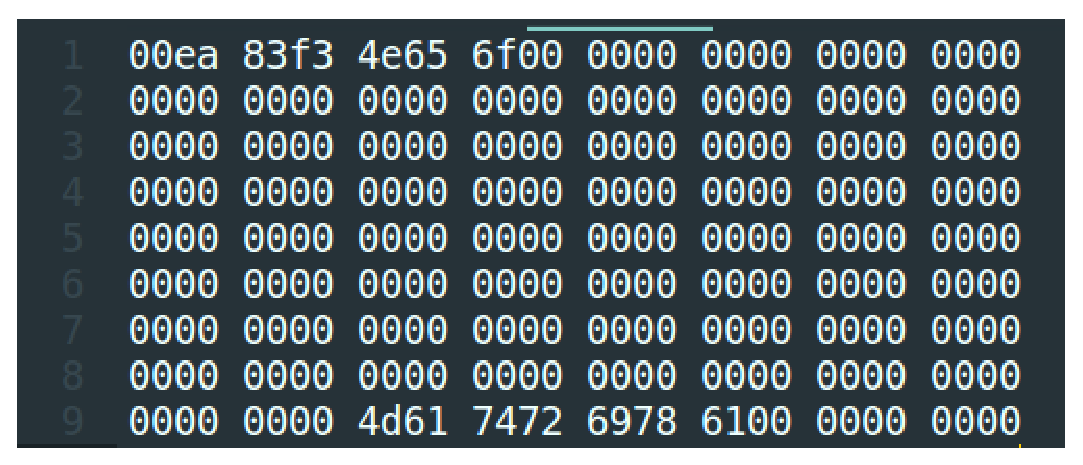
\includegraphics[width=\textwidth]{10.eps}~\\
\clearpage
~\\
\textbf{git checkout "nume"} - face switch la branchul "nume".~\\
\textbf{git branch -u upstream/name} - face track la branchul indicat din
branchul curent.~\\
\textbf{git branch -u upstream/name "nume" } - face track din branchul "nume"
la branchul indicat.~\\
\textbf{git branch --track "name" upstream/name} - creeaza branchul "name" si ii face track
la branchul indicat.~\\
\textbf{git branch --unset-usptream} - scoate trackingul la branchul in care ne
aflam.~\\
~\\
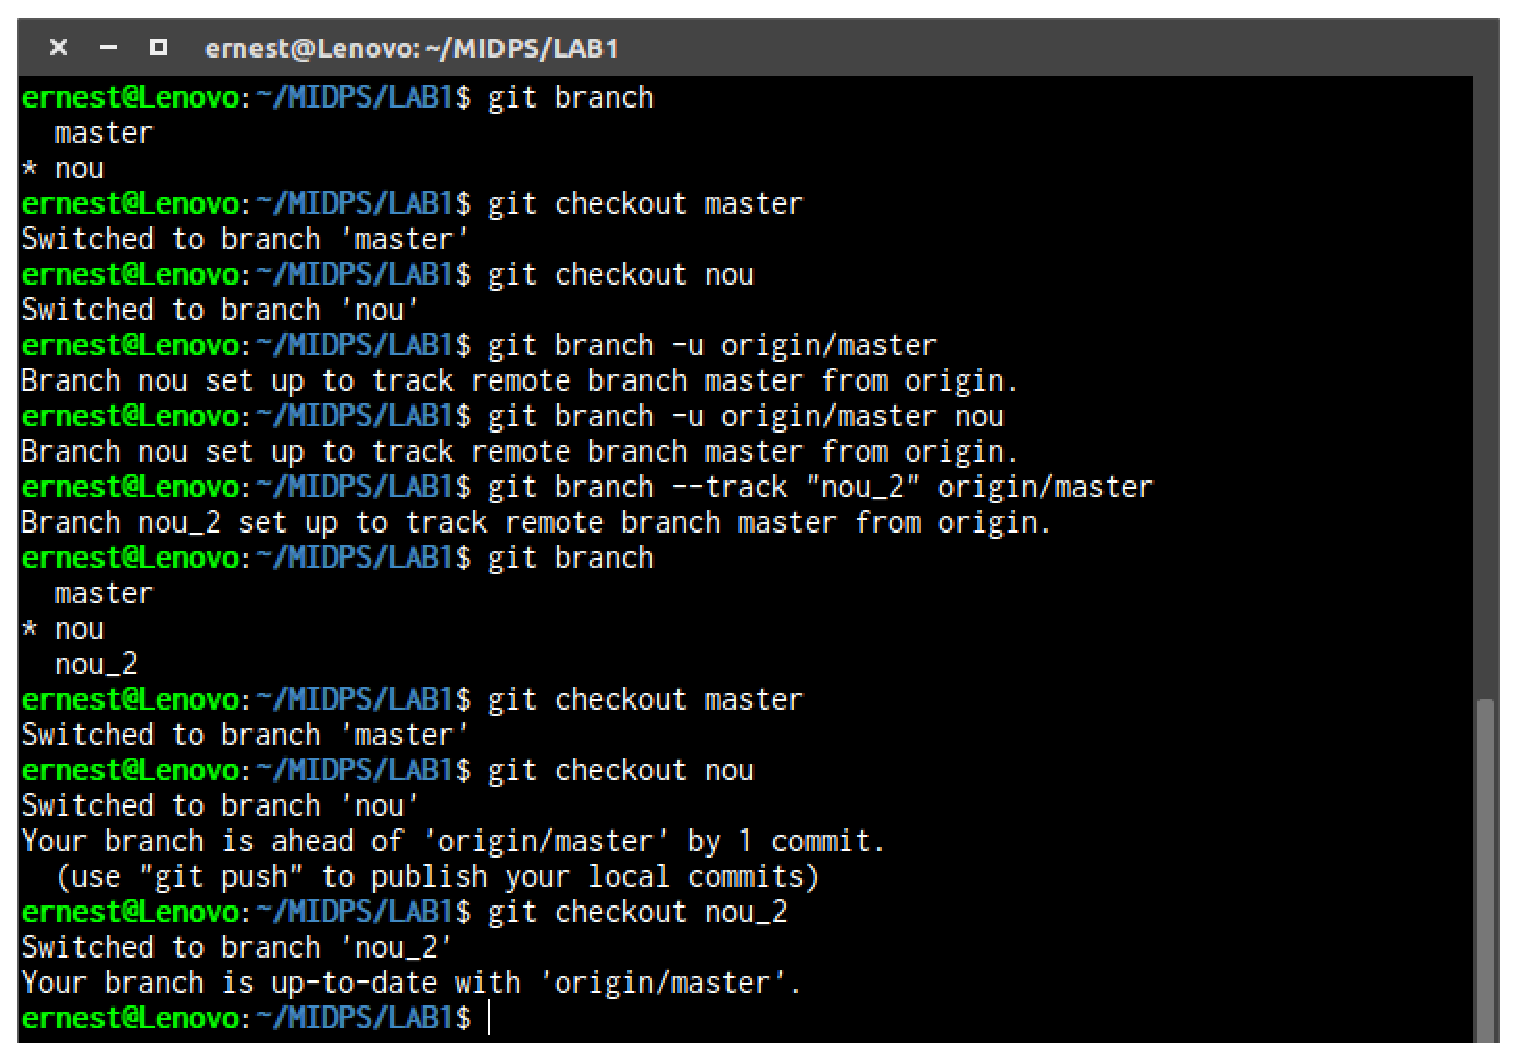
\includegraphics[width=\textwidth]{12.eps}~\\
~\\
